\documentclass[12pt]{article}
\usepackage{polski, graphicx, amsmath, caption, subcaption, float, indentfirst, booktabs, hyperref}

\title{
    Dokumentacja projektu EasyVENTER \\
    \large Bazy Danych 1
    }
\author{Patryk Będkowski \and Łukasz Szarejko \and Szymon Skarzyński \and Marcin Grabysz}
\date{\today}

\begin{document}

\maketitle

\section{Ogólny opis rozwiązania}

    Koncepcja projektu została zainspirowana naszymi doświadczeniami z kupowania biletów na mecz Polska - Węgry w październiku 2021. System działał niesprawnie, był nieczytelny i ostatecznie musieliśmy kupić bilety w innym sektorze, niż planowaliśmy. Mając w pamięci te doświadczenia, postanowiliśmy zainteresować się tym tematem i stworzyć aplikację do kupowania biletów na wydarzenia sportowe i kulturalne. Stworzona przez nas baza danych i obsługująca ją aplikacja \textbf{EasyVENTER} (napisana w Javie przy użyciu biblioteki Swing) umożliwia wymianę informacji między organizatorami wydarzeń oraz klientami kupującymi bilety.
    
    \subsection{Możliwości organizatora}
        
        Użytkownik zalogowany jako organizator ma możliwość tworzenia nowych wydarzeń oraz ich późniejszego modyfikowania. Tworząc wydarzenie, organizator podaje nazwę wydarzenia, datę i czas rozpoczęcia oraz adres (ulica, miasto oraz kraj z obsługiwanej puli krajów). Aplikacja umożliwia również dywersyfikację cen, dlatego organizator może podzielić pulę biletów na sektory (tu kolejna inspiracja kupowaniem biletów na Stadionie Narodowym) i przypisać każdemu z sektorów unikalną nazwę, liczbę miejsc oraz bazową cenę.
        \\ \par
        Modyfikując wydarzenie, organizator może zmienić jego datę oraz adres. Opcja modyfikowania puli biletów i ich cen nie jest dostępna, żeby nie powodować konfliktów w sytuacjach, gdy klienci kupili już bilety na pewne wydarzenie.
        
    \subsection{Możliwości klienta}
    
        Użytkownik zalogowany jako klient może przeglądać dostępne wydarzenia i kupować bilety z dostępnej puli w wybranym sektorze. Jeden klient ma możliwość kupienia maksymalnie dziesięciu biletów w każdej z kategorii: dorosły, dziecko, VIP (kategorie różnią się ceną). 
        \\ \par
        Klient może także przeglądać wydarzenia, na które posiada przynajmniej jeden bilet i anulować dowolną liczbę biletów. Anulowanie ostatniego biletu jest równoznaczne z rezygnacją z całego zamówienia, ale użytkownik może zakupić bilety na to wydarzenie ponownie, znajdując je wśród dostępnych wydarzeń.
    
    \subsection{Rejestracja użytkownika}
    
        Oprócz obsługi przykładowych użytkowników dostępnych od początku w bazie danych, aplikacja umożliwa dodawanie nowych klientów oraz organizatorów. Dane pobierane podczas rejestracji to: imię, nazwisko, login, hasło, adres email oraz telefon; klient dodatkowo: płeć, data urodzenia; organizator dodatkowo: nazwa firmy.
        
\section{Najważniejsze tabele}

    Cała baza zawiera 15 tabel - to trochę więcej, niż byłoby konieczne i zgodne z intuicją, jednak podeszliśmy do projektu z myślą o ćwiczeniu i opanowaniu tworzenia oraz modyfikowania baz danych. 

        \begin{center}
        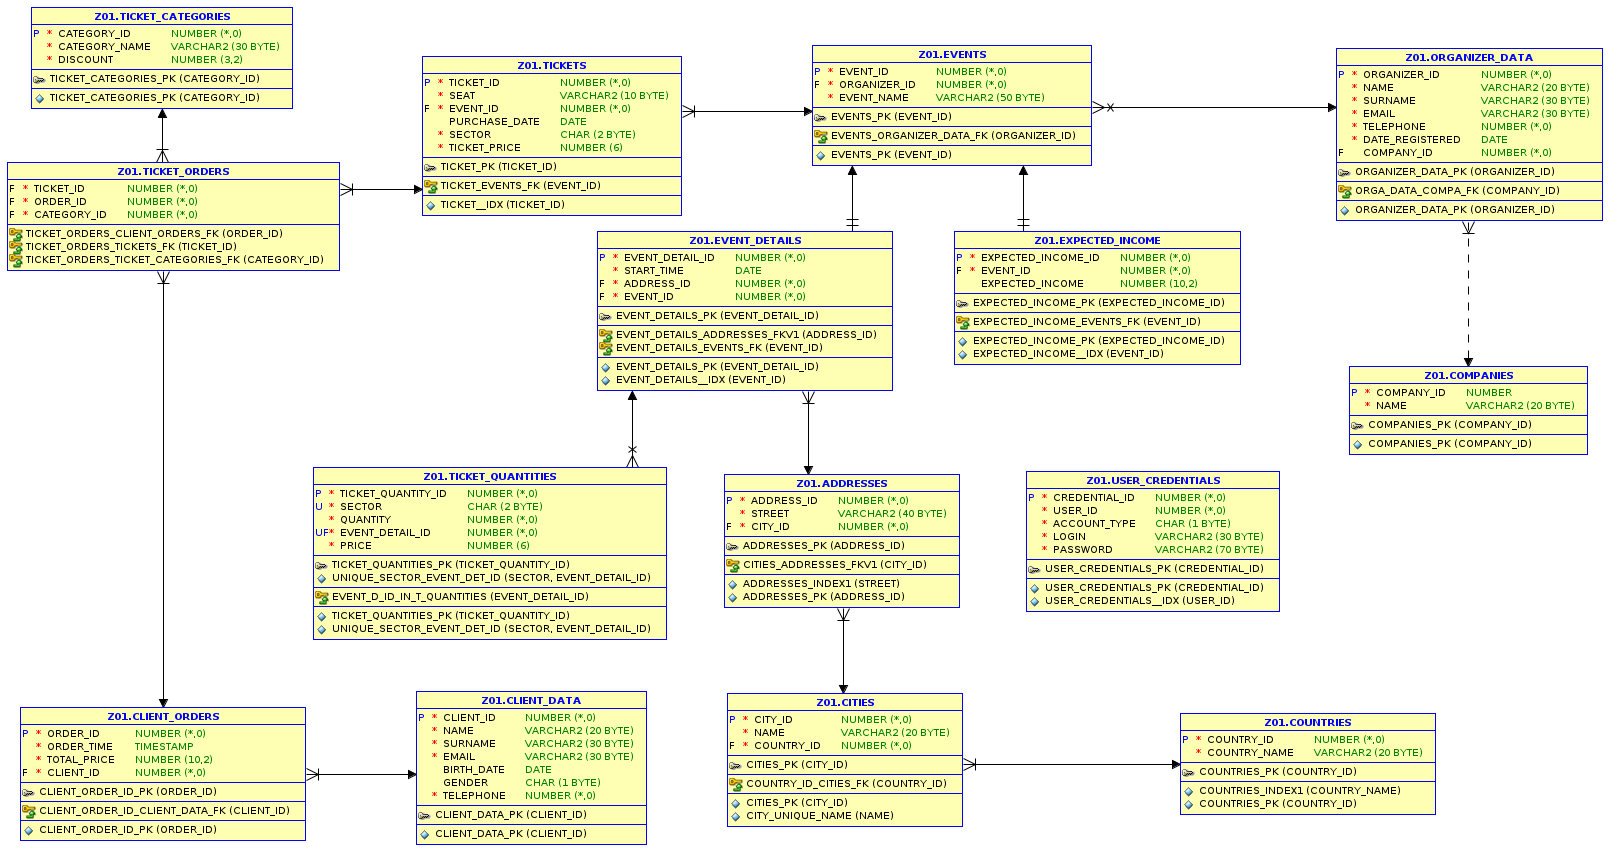
\includegraphics[width=\textwidth]{EASYVENT_DATABASE_RELATIONAL_MODEL.png}
        \captionof{figure}{Model relacyjny wszystkich tabel}
        \end{center}

    Najważniejsze tabele są opisane poniżej:
    
    \subsection{Events}
        
        Tabela łącząca ID wydarzenia z jego nazwą i ID organizatora. ID wydarzenia umożliwia uzyskanie szczegółów wydarzenia oraz informacji o kupionych biletach.
    
    \subsection{Tickets}
    
        Każdy wiersz tabeli reprezentuje jeden bilet - bilet przechowuje ID, ID wydarzenia, numer siedzenia, sektor, cenę i datę zakupu.
        
    \subsection{Ticket\_orders}
    
        Tabela przechowuje zamówienia - każde zamówienie polega na kupieniu pewnej ilości biletów różnych kategorii na jedno wydarzenie przez jednego klienta.
        
    \subsection{Client\_data}
    
        Tabela przechowuje informacje o użytkownikach będących klientami: ID, imię, nazwisko, email, data urodzenia, płeć, telefon.
        
    \subsection{Organizer\_data}
    
        Tabela przechowuje informacje o użytkownikach będących organizatorami: ID, imię, nazwisko, email, telefon, data zarejestrowania, ID firmy.
        
\section{Opis funkcji i procedur w bazie danych}         

    \subsection{Funkcje}
    
        \begin{itemize}
            \item {\tt calculate\_total\_price} - funkcja ta odpowiada za obliczanie całkowitej ceny zamówienia złożonego przez klienta. Pobiera podstawową cenę biletu, mnożnik zależny od wybranej kategorii oraz aktualny koszt zamówienia, a następnie liczy cenę biletu w danej kategorii i zwraca aktualny koszt zamówienia powiększony o cenę rozważanego biletu.
            \item {\tt get\_company} - funkcja ta zwraca nazwę firmy, do której należy organizator, którego login został podany jako argument funkcji.
        \end{itemize}
        
    \subsection{Procedury}
    
        \begin{itemize}
            \item {\tt buy\_ticket} - głównym zadaniem procedury buy\_ticket stanowi zakupienie pojedyńczego biletu dla danego zamówienia klienta.
            
            Procedura przyjmuje 7 argumentów, z czego dwa dotyczą danych klienta, kolejne 3 dotyczą typu biletu do zakupienia, natomiast ostatnie 2 to kolejno numery ID zamówienia oraz zmienna typu OUT, która zwraca owy numer zamówienia.
            
            Architektura tej procedury polega na tym, że wykonuje się ona kilka razy, jeżeli klient w ramach jednego zamówienia zakupi więcej niż jeden bilet. Przy pierwszym wywołaniu, do procedury przekazywany jest nieistniejący numer zamówienia. W takim przypadku system bazy danych wykrywa to i tworzy nowe zamówienie, którego id jest następnie zwracane na zewnątrz. Aplikacja w Javie, odbiera ID owego zamówienia i wywołuje tę procedurę ponownie, lecz teraz z istniejącym numerem zamówienia, dzięki czemu możliwe jest kupienie kilku biletów w ramach jednego zamównienia.

            Przy zakupie wymaganego biletu, sprawdzane są założenia dotyczące, czy specyfikacja biletu jest poprawna, tzn. czy owy event, kategoria biletu istnieją, a także czy klient jest zarejestrowany w systemie. Procedura wywołuje również funkcję calculate\_total\_price, która oblicza cenę zakupionego biletu.
            
            \item {\tt add\_event} - procedura ta dodaje nowe wydarzenie do bazy danych, uzupełniając przy tym wymagane tabele, takie jak adresses, event\_details itp.
            \item {\tt remove\_ticket} - usuwa bilet z zamówienia klienta, zmieniając przy tym koszt danego zamówienia.
            \item {\tt register\_organizer} - dodaje organizatora do bazy danych.
            \item {\tt register\_client} - analogicznie jak register\_organizer, tylko dla klienta.
            \item {\tt edit\_event} - porcedura ta edytuje możliwe do edycji informacje o wydarzeniu. Możliwe do edycji są czas i miejsce wydarzenia.
            \item {\tt cancel\_event} - usuwa dane wydarzenie z bazy danych. Ze względu na problem, przy projekcie z PAPu, jako jedyna nie jest używana w aplikacji. Jest jednak możliwością rozwoju projektu.
            \item {\tt add\_ticket} - dodaje bilet do nowo utworzonego wydarzenia, który może zostać zakupiony
            \item {\tt add\_ticket\_quantity} - ustawia ilość biletów dla danego sektora i o danej cenie dla konkretnego wydarzenia.
            \item {\tt add\_ticket\_to\_order} - łączy zakupiony bilet ze złożonym przez klienta zamówieniem poprzez wpis do tabeli ticket\_orders.
        \end{itemize}
        
\section{Wygląd interfejsu graficznego}

    Poniżej przedstawione jest kilka przykładowych ujęć interfejsu graficznego aplikacji EasyVENTER.
    
    \begin{center}
    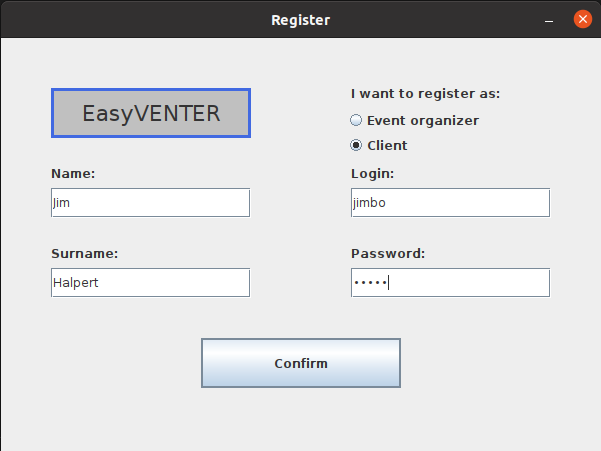
\includegraphics[width=\textwidth]{Registration_frame.png}
    \captionof{figure}{Ekran rejestracji użytkownika}
    \end{center}
    
    \begin{center}
    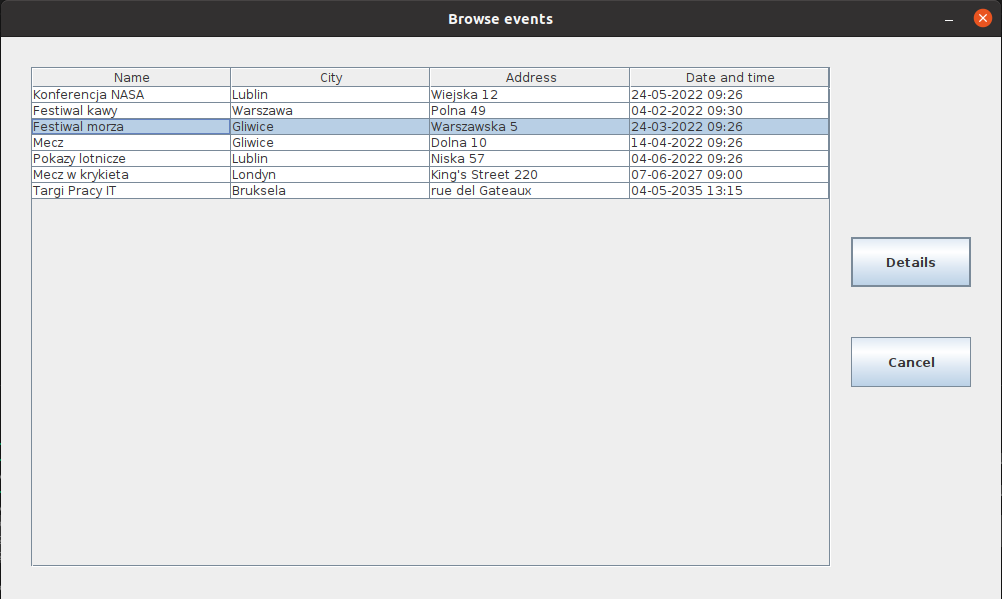
\includegraphics[width=\textwidth]{Browse_event_frame.png}
    \captionof{figure}{Ekran przeglądania dostępnych wydarzeń}
    \end{center}
    
    \begin{center}
    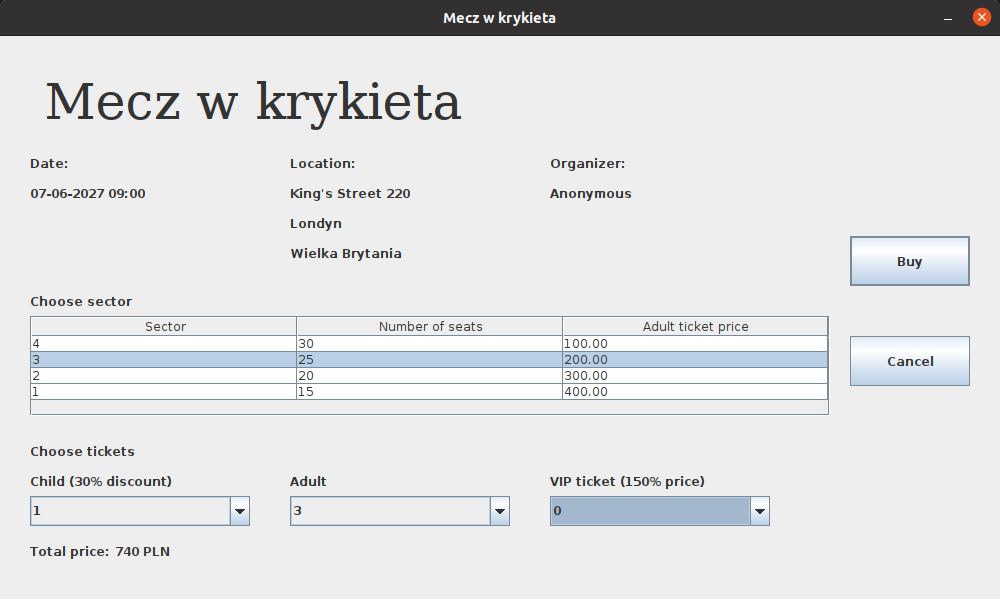
\includegraphics[width=\textwidth]{Event_details_frame.png}
    \captionof{figure}{Ekran kupowania biletów na wydarzenie}
    \end{center}
        
\section{Analiza rozwiązania}

    \subsection{Ograniczenia}
        
        Baza danych została zaprojektowana w taki sposób, aby wprowadzić przejrzysty podział informacji. Wyróżnić możemy pewne grupy tabel, które ułatwiają przechowywanie powiązanych ze sobą danych np. zamówienia klientów ({\tt client\_orders}) oraz informacje o poszczególnych biletach w tych w zamówieniach ({\tt ticket\_orders}). Zaletą takiego rozwiązania jest przechowywanie powiązanych ze sobą informacji w mniej zgrupowany sposób. Wadą natomiast jest potrzeba budowy bardziej skomplikowanych zapytań w celu uzyskania dostępu do większej liczby informacji jednocześnie. W rozwijanym przez nas programie wykorzystującym ową bazę, takowe zapytania stanowią zdecydowaną mniejszość, co przeważyło nad decyzją wprowadzenia większej ilości tabel.
    
    \subsection{Możliwości rozwoju}
    
        Dzięki tabeli {\tt expected\_income} możemy w przyszłości wzbogacić nasz program o udostępnianie oganizatorom informacji, jakiego przychodu mogą się spodziewać przy obecnym obłożeniu ich wydarzenia.
        \\ \par
        W tabeli {\tt ticket\_categories} możemy wprowadzić więcej kategorii biletów, jeśli zajdzie taka konieczność - bazowo udostępniliśmy tylko trzy kategorie (dorosły, dziecko, VIP), ale można sobie wyobrazić dużo więcej; wystarczy choćby spojrzeć na kilkanaście zniżek oferowanych przez PKP: uczniowska, studencka, kombatancka, itp.  
        
    \subsection{Inne wnioski}
    
        Dzięki wydzieleniu loginów i haseł do osobnej tabeli {\tt user\_credentials} nie ma potrzeby pobierania wszystkich danych użytkowników podczas logowania. Inaczej jest podczas rejestracji, ale też logowanie użytkownika jest operacją występującą znacznie częściej niż rejestrowanie nowego.
        \\ \par
        Mamy wrażenie, że baza danych jest przejrzysta i łatwa w użytkowaniu. Wiele tabel zapewnia rozproszenie informacji, ale programista pracujący z tabelą intuicyjnie odnajdzie potrzebne dane dzięki klarownym nazwom i dostępnemu diagramowi relacyjnemu. Użytkownik ma do dyspozycji prosty w obsłudze i estetyczny interfejs.
        
\end{document}
